\documentclass[conference]{IEEEtran}
\usepackage{graphicx}
\usepackage{subfigure}
\usepackage[utf8]{inputenc}
\usepackage{tikz}
\usetikzlibrary{shapes.geometric, arrows}
\usepackage{caption}
\usepackage{tfrupee}
\usepackage{subfig}
\usepackage{subcaption}
\usepackage{hyperref}
\usepackage{parselines} 
\usepackage{float}



\hyphenation{op-tical net-works semi-conduc-tor}

\makeatletter
\newcommand{\linebreakand}{
  \end{@IEEEauthorhalign}
  \hfill\mbox{}\par
  \mbox{}\hfill\begin{@IEEEauthorhalign}
}
\makeatother

\begin{document}

\title{
Intelligent Traffic Control Model Checking Using UPPAAL
}


\author{
\IEEEauthorblockN{
Mohit Awachar
}
\IEEEauthorblockA{
Department of Information Technology\\
National Institute of Technology Karnataka\\
Surathkal-575025, India \\
mohit.191it231@nitk.edu.in
}
\and
\IEEEauthorblockN{
Anshul Patel
}
\IEEEauthorblockA{
Department of Information Technology\\
National Institute of Technology Karnataka\\
Surathkal-575025, India.\\
anshulpatel.191it208@nitk.edu.in
}
\linebreakand
\IEEEauthorblockN{
Rakshit Kulkarni
}
\IEEEauthorblockA{
Department of Information Technology\\
National Institute of Technology Karnataka\\
Surathkal-575025, India\\
rakshitkulkarni.191it245@nitk.edu.in
}
\and 
\IEEEauthorblockN{
Kiran Kumar J M
}
\IEEEauthorblockA{
Department of Information Technology\\
National Institute of Technology Karnataka\\
Surathkal-575025, India\\
 kirankumarjm.191it126@nitk.edu.in
}
}

\maketitle

\begin{abstract}

This paper focuses on model checking of a Traffic Light System. This paper is an extension of the paper Uppaal Stratego for Intelligent Traffic Lights published in France in 2017. In the base paper the plan was to find an optimal strategy for minimum traffic. Here the main focus is on model checking of traffic light systems and verifying if all the states are reachable and if all the safety requirements are satisfied. Uppaal is the tool used for model checking in this work. It is an integrated tool for modeling, simulation and verification of real-time systems( in this case the traffic light system).
\\

\rule{0.1cm}{0pt} Keywords--- traffic lights, model checking, uppaal , verification and validation.
\end{abstract}

\IEEEpeerreviewmaketitle

\section{Introduction}

Traffic lights also called traffic lamps or signal lights have the responsibility to manage the flow of traffic at junctions or intersections of roads. A typical traffic light has three colors namely red indicating to stop, green indicating the vehicle can cross the junction and yellow or orange means the signal is about to switch to green or red. Traffic lights play a very crucial role in flow of traffic every day and it prevents or at least reduces many vehicle crashes that can happen otherwise. It ensures a safe and orderly flow of traffic on roads and highways. In addition, traffic lights also ensure safety of pedestrians crossing the road. The signal ensures that pedestrians also get a share or road without worrying about safety. This paper focuses on the model checking and verification of safety conditions of traffic light systems.
\\

Model checking is a method for checking if a finite-state model of a system satisfies the specifications provided. Traffic-Light Control System is the system under consideration with respect to this paper. Traffic-Light system being a safety critical system, it’s failure can lead to heavy loss of property as well as life. To solve this problem algorithmically, both models of the Traffic Light System and it’s specifications are formulated in precise mathematical language. Now that the problem is formulated as a task in logic, the model checking tool needs to verify if the logical property is satisfied for the given logical formula. A simple model-checker can be a tool verifying whether a formula in propositional logic is satisfied by a system or not.
\\

Symbolic Model Checking(SMC) is a formal verification  technique which does not require any user assistance. In SMC, it is possible to verify an implementation by modelling it as an finite-state transition graph to check if it satisfies given specifications. This is done by giving some properties of temporal logic.
\\

Many tools are available for model checking like NuSMV, PAT, Prism, etc. In this implementation we have used Uppaal stratefor for model checking. It is an integrated tool for modeling, verification and validation of real-time systems. The system is modelled as a network of timed-automata. More information about this tool is discussed in the methodology part.


\section{Literature Survey}

In this paper [1] the authors have done a simulation of traffic in sumo and use uppaal as backend tool to find the optimal strategy to minimize the waiting time.  
\\

In this paper [2] the authors have extended the work in [1]Uppaal Stratego for Intelligent Traffic Lights. The authors considered multiple traffic lights and used UPPAAL Stratego to find the optimal stratego by bringing a coordination between data collected by the signals to reduce the traffic.
\\

All the papers were focusing on finding the optimal strategy to find the optimal strategy to reduce traffic. None of the papers did the model checking of the traffic light system and verified it’s safety and reachability properties. We aim to do the same in this paper.

\section{Problem Statement}

Intelligent Traffic Control Model Checking using UPPAAL. 

\section{Proposed Work}
\begin{enumerate}
    \item Define the Traffic Light System
    \item Model the Traffic Light System in UPPAAL
    \item Simulate the Flow of traffic and Pedestrians in UPPAAL
    \item Express Reachablitiy, Safety, Deadlock and other properties in UPPAAL
    \item Verification of Properties in UPPAAL
    
\end{enumerate}
\\
\begin{figure}[H]
    \centering
    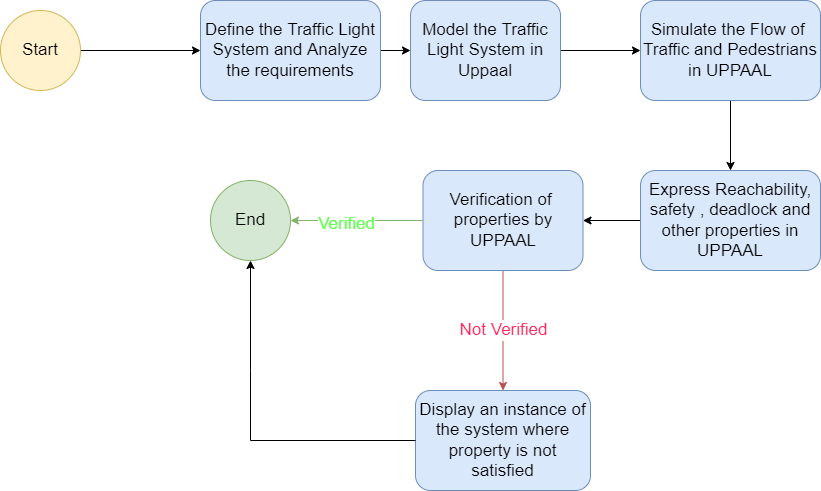
\includegraphics[width=0.4\textwidth]{FlowChart.drawio.png}
    \caption{The Traffic Light.}
\end{figure}



\section{Methodology}

Let’s look at the modelling tool Uppaal Stratego first.
\\

\noindent \textbf{Uppaal Stratego  :}
Uppaal is an integrated tool for modeling, simulation and verification of real-time systems. This tool is developed by joint contribution of the Basic Research in Computer Science at Aalborg University in Denmark and the Department of Information Technology at Uppsala University in Sweden. Typical applications are systems where timing is important such as real-time controllers and communication protocols.
\\

\noindent Uppaal consists of three major parts
\begin{itemize}
    \item \textbf{Description Language :} This is a non-deterministic language with different data types. It serves as a design language to describe our system behavior as a network of automata. The language also supports clock and data variables.
    \item \textbf{Simulator :} This is a validation tool which enables examination of possible dynamic execution of the system under consideration.
    \item \textbf{Model-checker :} This checks for the reachability properties by exploring the state of the system. It also checks the invariant properties.
\end{itemize}
\\

\noindent In the Uppaal application one can see three portions 
\begin{itemize}
    \item \textbf{Editor :} 
In the editor section of UPPAAL the user can define various states of his system. The user can create a template for a particular subsystem and define various states and transition among them for the subsystem. In the global declarations one can define global variables. In the system declarations, users can define multiple or single instances of the templates created.The various systems can be synchronized with the help of channels. The time can be monitored with the help of clocks.
\item \textbf{Simulator :} 
In this section, the user can see all the instances of the subsystem created by him.  In the top left corner the possible transitions are shown. In the bottom right corner the detailed history of all transitions is shown. In the top right corner (i.e. the major portion) all the state diagrams of all instances are shown and the current states are highlighted. Other than this all global and local variables are also visible.
\item \textbf{Verifier :} 
In this section the user can insert the properties he/she is interested to verify for the system.
\end{itemize}

\\
\noindent \textbf{The Traffic Light system : }
We are considering a traffic light system for model checking. The system is an intersection of two perpendicular roads and a traffic light present at the intersection. As shown in the figure below, the two perpendicular roads NS and EW intersect at a point TL(Traffic Light). The system also has crossings for the pedestrians.
\\

The traffic light has three phases namely green , red and yellow for both the lanes. Following are the rules we follow for the traffic light.
\\
\begin{figure}[H]
    \centering
    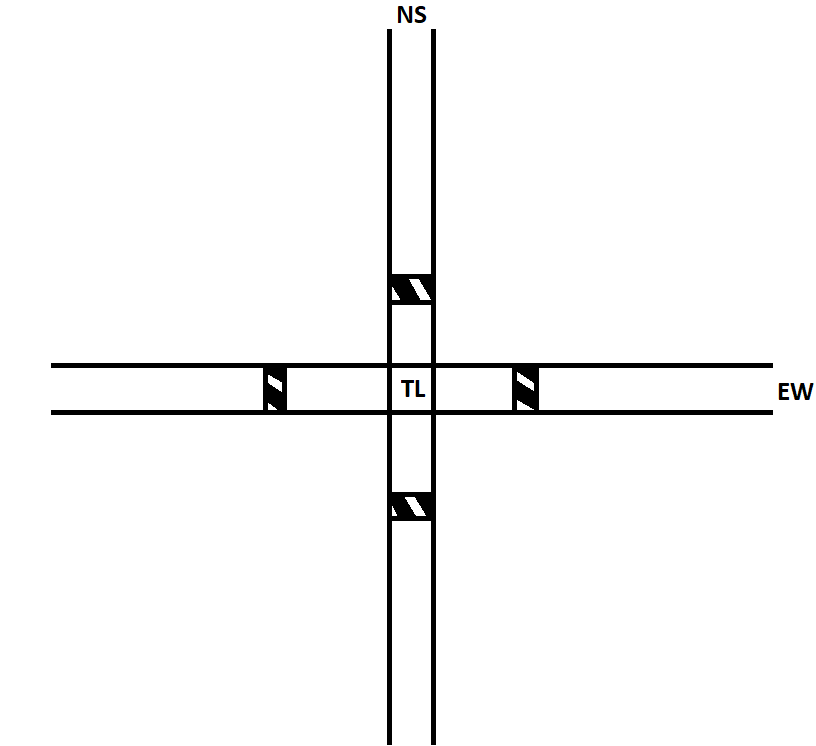
\includegraphics[width=0.5\textwidth]{road.png}
    \caption{The Traffic Light.}
\end{figure}
\\
\begin{itemize}
    \item When a lane is red the vehicle can’t cross. When the lane is green, the vehicle has a choice to cross or wait.
    \item Once a lane(NS or EW) is made green, the lane remains green as long as some vehicle is waiting in the lane
    \item Once both the lanes are red the pedestrians can cross the road. The lanes will remain red until all the pedestrians cross the lane.
    \item The lane have a fixed timer of 5 seconds for the yellow signal.
    \item The traffic lights go in order green-yellow-red-yellow-green.

\end{itemize}


\\
\noindent \textbf{The UPPAAL Model :}
We define 4 templates for our system in UPPAAL.
\\
\begin{enumerate}
    \item The Traffic Light
    \begin{figure}[h]
        \centering
        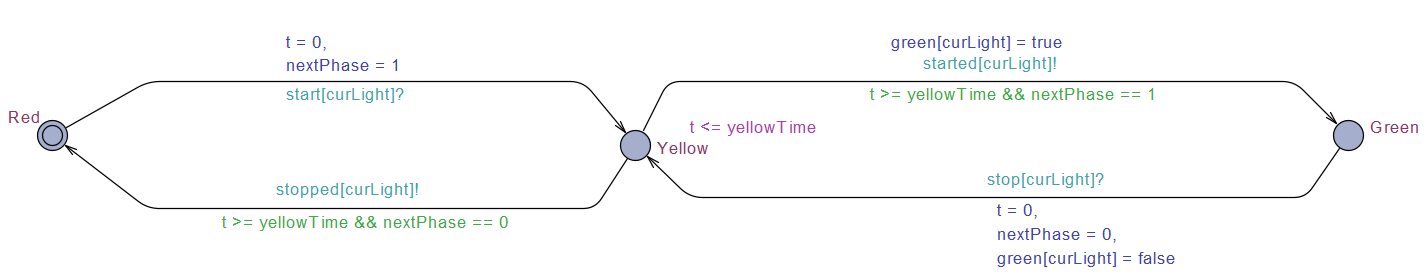
\includegraphics[width=0.4\textwidth]{Fig 4.png}
    \caption{The Traffic Light.}
    \end{figure}
    \\
    \textbf{Parameters :} curLight and yellowTime
    \\
    \textbf{Local Declarations :} clock and nextPhase
    \\
    \textbf{Possible States :}
    \begin{itemize}
        \item Red : The vehicle can’t cross and the pedestrians are free to cross the road.
        \item Yellow : This is the phase between green and red and is encountered two times in a cycle. The phase has an invariant that the subsystem must remain in this state for 5 seconds each time.
        \item Green : The vehicles in the current lane can cross and the pedestrians have to wait.

    \end{itemize}
    \\
    At the start the signal is in Red state. The signal can move to Yellow state from here once it receives the signal ( from channel start[curLight] ) from the controller. During this transition the controller updates t=0 and nextPhase=1. In the Yellow state, the signal must stay for yellowTime and then the signal has two options namely Green or Red State. When nextPhase is one the signal moves to Green state and moves to Red state otherwise. During these transitions, a signal( started[curLight] or stopped[curLight] ) is sent to the controller. When the TrafficSignal is in Green state, it can move to Yellow state once it receives the signal( from channel stop[curLight] ) from the controller. During this transition, time and nextPhase are updated to 0.
    \\
    
    \item The Vehicle 
    \begin{figure}[H]
        \centering
        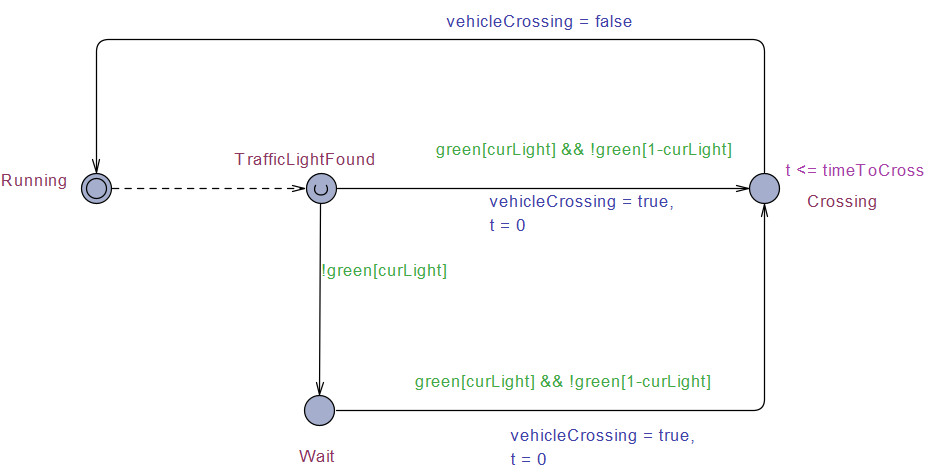
\includegraphics[width=0.5\textwidth]{Fig 2.png}
    \caption{The Vehicle.}
    \end{figure}
    \\
    \textbf{Parameters :} curLight and timeToCross
    \\
    \textbf{Local Declarations :} clock
    \\
    \textbf{Possible States :}
    \begin{itemize}
        \item Running : The vehicle is freely running on free roads.
        \item TrafficLightFound : The vehicle encountered a traffic light.
        \itme Wait : The vehicle is waiting in front of the traffic light.
        \item Crossing : The vehicle is crossing the junction.
    \end{itemize}
    \\
    At the start, the vehicle is in Running state. When the vehicle encounters a traffic light it is shifted to TrafficLight Found state. This state is marked as urgent meaning one must take a transition here. If the lane is green the Vehicle moves to Crossing state else it moves to Wait state. The vehicle can stay in the Crossing state for time less than timeToCross and after this it moves to Running state again. The Vehicle can move from Wait to Crossing when the lane is green.
    \\
    
    \item The Pedestrian
    \begin{figure}[H]
        \centering
        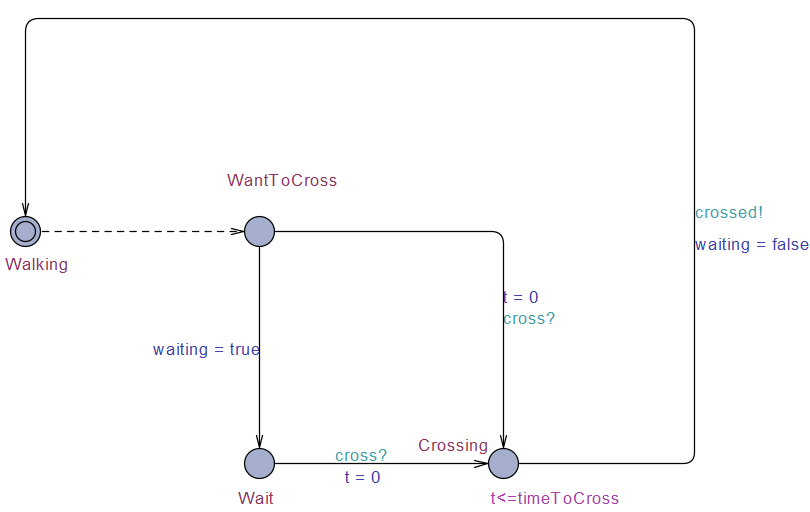
\includegraphics[width=0.5\textwidth]{Fig 3.png}
    \caption{The Pedestrian.}
    \end{figure}
    \\
    \textbf{Parameters :} curLight and timeToCross
    \\
    \textbf{Local Declarations :} clock
    \\
    \textbf{Possible States :}
    \begin{itemize}
        \item Walking : The pedestrian is walking freely on a footpath.
        \item WantToCross : The pedestrian encounters a road junction.
        \item Wait : The pedestrian is waiting for vehicles to pass to cross the junction.
        \item Crossing : The pedestrian is crossing the junction.

    \end{itemize}
    \\
    Initially the Pedestrian is in Walking state. When he/she encounters a junction he/she changes to WantToCross state. At this stage if we receive a cross signal from the controller the Pedestrian can move to Crossing State. Else the Pedestrian moves to Wait state. From the Wait state, The Pedestrian moves to Crossing state on encountering cross signal from the Controller. The Pedestrian can stay in Crossing state for less time less than  timeToCross and then moves to Walking state again. When this transition is in progress a signal is sent to the controller that the Pedestrian has crossed the junction.
    \\
    
    
    \item The Controller
    \begin{figure}[H]
        \centering
        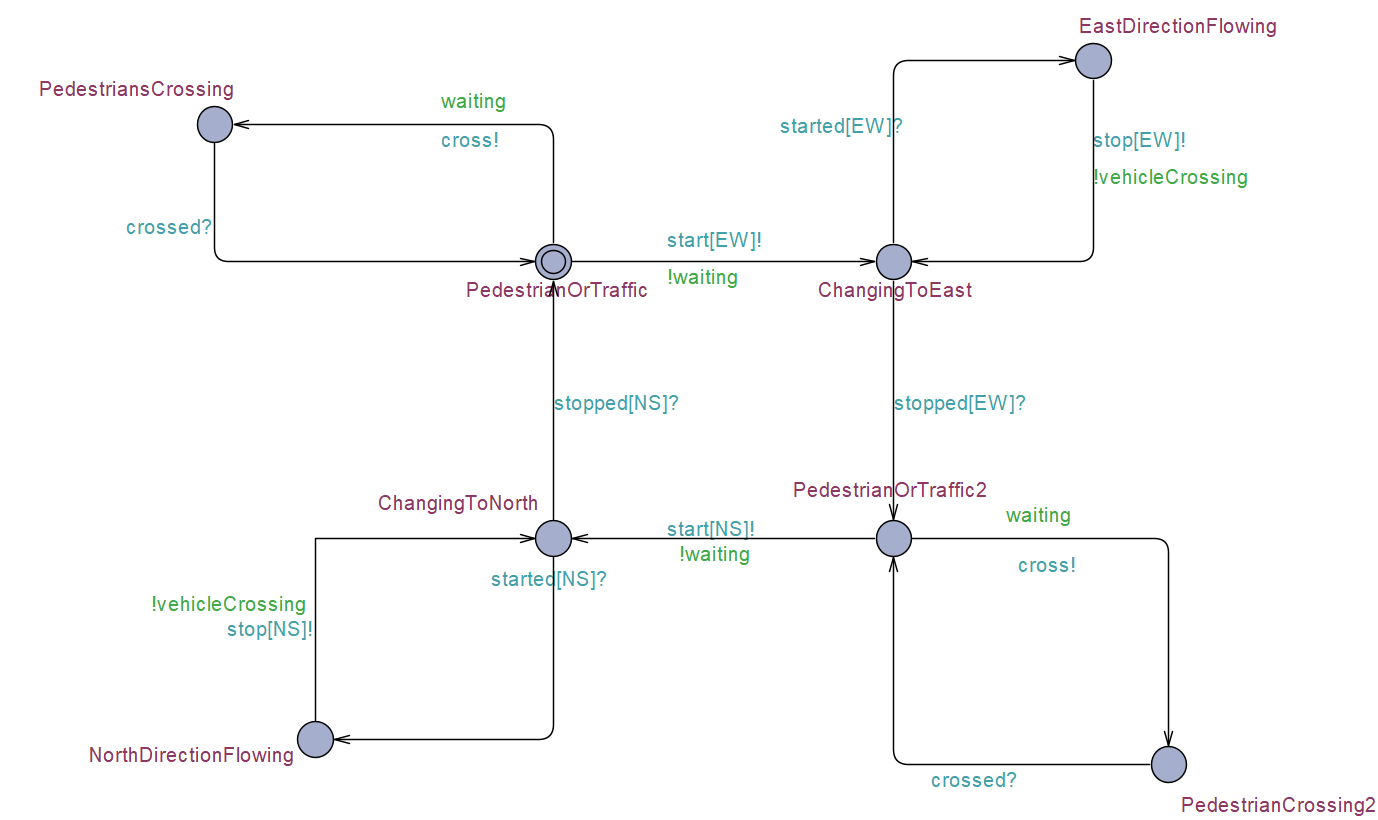
\includegraphics[width=0.5\textwidth]{Fig 5.png}
    \caption{The Controller.}
    \end{figure}
    \\
    \textbf{Parameters :} None
    \\
    \textbf{Local Declarations :} None
    \\
    \textbf{Possible States :}
    \begin{itemize}
        \item PedestriansCrossing / PedestriansCrossing2 : The pedestrians are crossing the junction.
        \item PedestrianOrTraffic / PedestrainOrTraffi2 : The controller can allow Pedestrians or vehicles to cross
        \item ChangingToEast : The flow of vehicles along EW lane can start/stop
        \item ChangingToNorth : The flow of vehicles along NS lane can start/stop
        \item EastDirectionFlowing : The EW lane is active
        \item NorthDirectionFlowing : The NS lane is active

    \end{itemize}
    \\
    The Controller is initially in PedestrainOrTraffic state. If a Pedestrian is waiting to cross, the Controller moves to PedestrainsCrossing state and when the Pedestrian crosses the road, the Controller returns to PedestianOrTraffic state. The other option in this state is to move to ChangingToEast state. When this transition is made a signal is sent to TrafficSignal. From ChangingToEast state, the Controller can move to EastDirectionFlowing allowing the flow of traffic in the EW lane. When no vehicle is crossing and waiting, the Controller can return to ChangingEast. The other option at this stage is to move to PedestianOrTraffic2 state. This state is similar to PedestrianOrTraffic state. From there the Controller moves to ChangingToNorth state. Again this state is similar to ChangingToEast only difference being here the flow of traffic is in NS direction. From this state, when flow of traffic is complete in NS direction, the Controller moves to its initial state( i.e PedestrianOrTraffic).
    \\
    
\end{enumerate}
\\
\noindent \textbf{Verification of Properties in Verifier}
\\
After the system is modelled in editor and simulated in simulator, the verification of reachability and safety properties is done in the verifier. More about these properties is discussed in the RESULT section.
\\
    




% \section{CONTRIBUTIONS}
% \\
% \begin{itemize}

%     \item Mohit Awachar
%     \begin{itemize}
%         \item Learn about UPPAAL.
%         \item Coordinate between all the templates.
%         \item Logic of Controller.
%         \item Queries for Safety Conditions.
%     \end{itemize}
    
%     \item Rakshit Kulkarni
%     \begin{itemize}
%         \item Learn about UPPAAL.
%         \item Decide the plan for which templates to make and how many instances of each template.
%         \item Logic of Controller.
%         \item Queries for Safety Conditions.
%     \end{itemize}
    
%     \item Anshul Patel
%     \begin{itemize}
%         \item Learn about UPPAAL.
%         \item Coordinate between all the templates.
%         \item Logic of Pedestrian.
%         \item Queries for Other Conditions.
%     \end{itemize}
    
%     \item Kiran Kumar J M
%     \begin{itemize}
%         \item Learn about UPPAAL.
%         \item Logic of  Vehicle.
%         \item Queries for Reachability Condition.
%     \end{itemize}
    
% \end{itemize}

\section{RESULTS AND FUTURE WORK}

In the simulator, we have the following subsystem.

\begin{figure}[H]
    \centering
    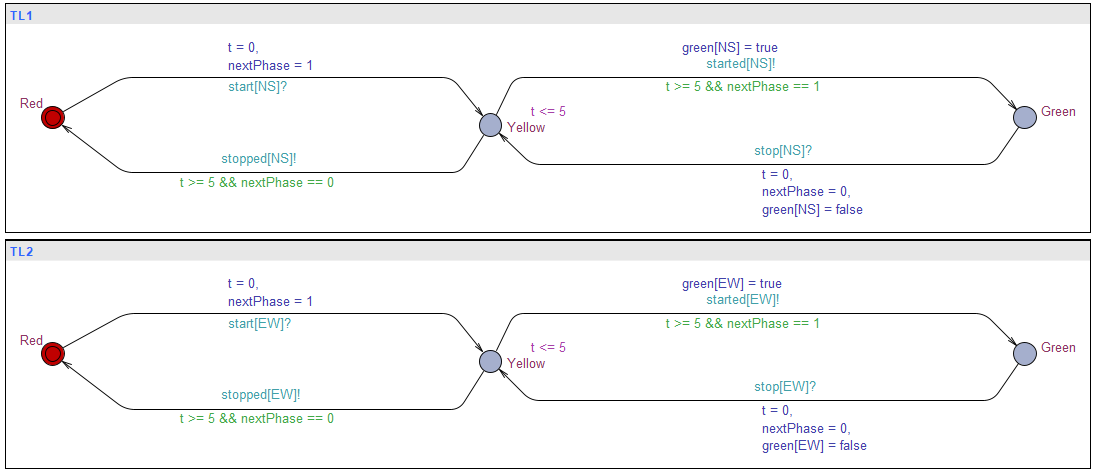
\includegraphics[width=0.5\textwidth]{Fig 6.png}
    \caption{The two traffic lights namely NS and EW}
\end{figure}
\\

\begin{figure}[H]
    \centering
    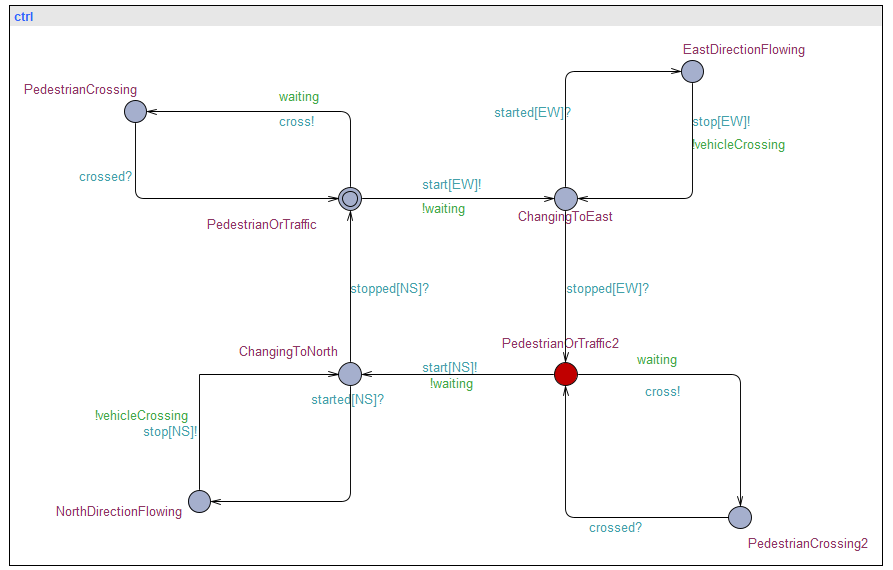
\includegraphics[width=0.5\textwidth]{Fig 7.png}
    \caption{The controller}
\end{figure}
\\

\begin{figure}[H]
    \centering
    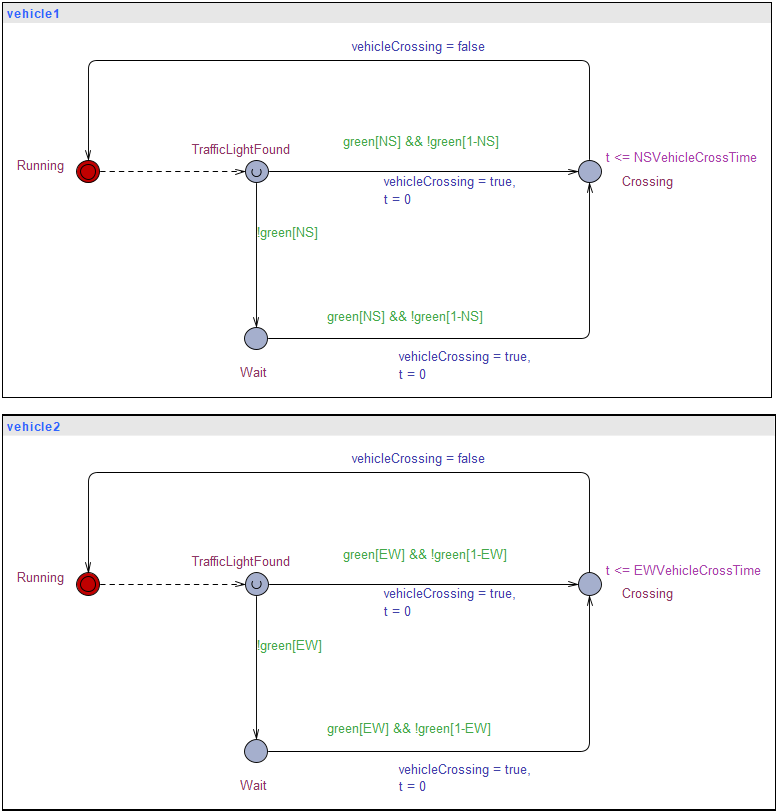
\includegraphics[width=0.5\textwidth]{Fig 8.png}
    \caption{The Vehicles}
\end{figure}
% \pagebreak
\\
Two vehicle types are vehicle1 flowing in the NS direction and vehicle2 in the EW direction.
\\
\begin{figure}[h]
    \centering
    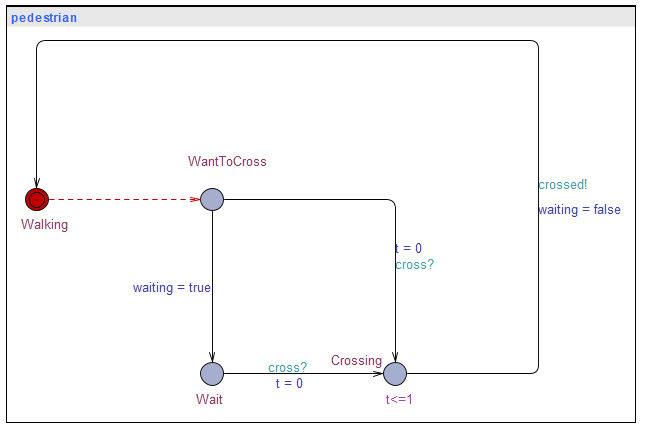
\includegraphics[width=0.5\textwidth]{Fig 9.png}
    \caption{The Pedestrian}
\end{figure}

\\
Finally we have the pedestrian.
\\

\noindent We verified the following properties for the system.
\\

\noindent \textbf{Reachability Properties :}
\begin{enumerate}

    \item For traffic Lights( TL1 and TL2 )
    \begin{enumerate}
        \item E$<>$ TL1.Red
        \item E$<>$ TL1.Green
        \item E$<>$ TL1.Yellow
        \item E$<>$ TL2.Red
        \item E$<>$ TL2.Green
        \item E$<>$ TL2.Yellow
    \end{enumerate}
    \\
    
    In these properties we aim to verify if all the states are reachable. So for each state of both the traffic signals we find if a path exists to reach there. All the above queries are satisfied.
    \\
    \item Pedestrian
    \begin{enumerate}
        \item E$<>$ pedestrian.Walking
        \item E$<>$ pedestrian.WantToCross
        \item E$<>$ pedestrian.Wait
        \item E$<>$ pedestrian.Crossing
    \end{enumerate}
    \\
    
    For pedestrian all the states ( i.e. Walking, WantToCross, Wait and Crossing are reachable). All the above properties are verified.
    \\
    
    \item Vehicle
    \begin{enumerate}
        \item E$<>$ vehicle1.Wait
        \item E$<>$ vehicle1.TrafficLightFound
        \item E$<>$ vehicle1.Crossing
        \item E$<>$ vehicle1.Running
        \item E$<>$ vehicle2.Wait
        \item E$<>$ vehicle2.TrafficLightFound
        \item E$<>$ vehicle2.Crossing
        \item E$<>$ vehicle2.Running
    \end{enumerate}
    \\
    For both the vehicles, all the states are reachable. All the above properties are verified.
    \\
    
    \item Controller
    \begin{enumerate}
        \item E$<>$ ctrl.ChangingToNorth
        \item E$<>$ ctrl.ChangingToEast
        \item E$<>$ ctrl.PedestrianOrTraffic
        \item E$<>$ ctrl.PedestrianOrTraffic2
        \item E$<>$ ctrl.PedestrianCrossing
        \item E$<>$ ctrl.PedestrianCrossing2
        \item E$<>$ ctrl.NorthDirectionFlowing
        \item E$<>$ ctrl.EastDirectionFlowing

    \end{enumerate}
    \\
    For the Controller, all the possible states are reachable so all the above properties are verified.
    
    
    
\end{enumerate}
\ \\
\noindent\textbf{Deadlock Property :}
\\
\indent A[] not deadlock
\\
\indent This means we did not get deadlock at any time. The property is also satisfied.
\\

\noindent\textbf{Safety Properties :}
\\

\begin{enumerate}
    \item \textbf{A[] not ( pedestrian.Crossing and (TL1.Green and TL2.Green) )}
    \\
    Pedestrian Crossing and both Traffic Lights are green; this condition is not possible at all times. The property is verified.
    \\
    \item \textbf{A[] not (TL1.Green and TL2.Green)}
    \\
    At all times both traffic lights can’t be green. The property is verified.
    \\
    \item \textbf{A[] not ( TL1.Yellow and TL2.Yellow)}
    \\
    At all times both traffic lights can’t be yellow. The property is verified.
    \\
    \item \textbf{A[] not ( (vehicle1.Crossing or vehicle2.Crossing) and pedestrian.Crossing )}
    \\
    A pedestrian can’t cross when either of the vehicle is crossing the road. The property is verified.
    \\
    \item \textbf{A[] not (vehicle1.Crossing and vehicle2.Crossing)}
    \\
    The vehicles in perpendicular lanes can’t pass at the same time. The property is verified.
    \\
    \item \textbf{A[] not ( vehicleCrossing and (ctrl.ChangingToEast or ctrl.ChangingToNorth) )}
    \\
    When a vehicle is passing through the junction, the controller must not change the traffic signal state. The property is verified.
\end{enumerate}
\ \\

\noindent \textbf{Other Properties :}
\\
\begin{enumerate}
    \item 
    \begin{enumerate}
    \item \textbf{E$<>$ vehicle2.Wait imply vehicle2.Crossing}
    \item \textbf{E$<>$ vehicle1.Wait imply vehicle1.Crossing}
    \end{enumerate}
    \\
    When a vehicle is waiting, it will get to cross eventually. The property is verified.
    \\
    \item \textbf{E$<>$ pedestrian.WantToCross imply pedestrian.Crossing}
    \\
    When a pedestrian wants to cross, he/she will get a chance to do so eventually. The property is verified.
    \\
    \item \textbf{E$<>$ (ctrl.NorthDirectionFlowing or ctrl.EastDirectionFlowing) imply (ctrl.PedestrianCrossing or ctrl.PedestrianCrossing2)}
    \\
    When vehicles are crossing then after some time eventually, pedestrians will get a chance. The property is verified.
    \\
    \item 
    \begin{enumerate}
        \item \textbf{E$<>$ ctrl.EastDirectionFlowing imply ctrl.NorthDirectionFlowing}
        \item \textbf{E$<>$ ctrl.NorthDirectionFlowing imply ctrl.EastDirectionFlowing}
    \end{enumerate}
    \\
    When one of the lanes is active, after some time eventually the other will be active. The property is verified.
    \\
    \item \textbf{A[] not (TL1.Red and TL2.Red)}
    \\
    At any time both traffic lights can't be red. But in this system they can be( when the pedestrians are crossing). So this property is \textbf{not satisfied} and the corresponding trace is visible in the simulator.
    \\
    \begin{figure}[h]
        \centering
        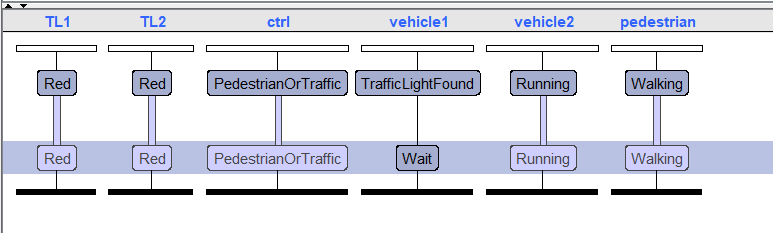
\includegraphics[width=0.5\textwidth]{Fig 10.png}
        \caption{The trace for both red signals}
    \end{figure}
\end{enumerate}
\section{CONCLUSIONS AND FUTURE WORK}
\ 

The traffic light system is modelled in UPPAAL with the help of state diagrams. The simulation is done in the simulator and one can manually move from one state to next according to simulation purposes. All the safety requirements, reachability properties and some other properties are properly analyzed and verified against the system using query language. The system passed all the safety and reachability requirements and no deadlock condition was encountered. The project was a very good learning experience for us. We get to learn about UPPAAL, verification and validation in Software Engineering.
\\

In the future, we plan to take a more complex traffic system with multiple roads at the intersection and allow different types of vehicles for modeling the system.
\\

\section{REFERENCES}
\

[1] Eriksen, Andreas & Huang, Chao & Kildebogaard, Jan & Lahrmann, Harry & Larsen, Kim & Muniz, Marco & Taankvist, Jakob. (2017). Uppaal Stratego for Intelligent Traffic Lights. \\

[2] B K, Thamilselvam & Kalyanasundaram, Subrahmanyam & Rao, M. (2019). Coordinated Intelligent Traffic Lights using Uppaal Stratego. 789-794. 10.1109/COMSNETS.2019.8711457. 
\\

\noindent About Uppaal :
\begin{itemize}
    \item \url{https://en.wikipedia.org/wiki/Model_checking}
    \item \url{https://uppaal.org/features/}
\end{itemize}
\ \\
\noindent Download UPPAAL at :
\begin{itemize}
    \item \url{https://uppaal.org/downloads/}
\end{itemize}

\end{document}